\subsection{Video Filter Application Using PREESM}
An actor network is constructed in PREESM that represents the video filter application. A network sketch is presented in Figure~\ref{sketch}.
\begin{figure}[h!]
\begin{center}
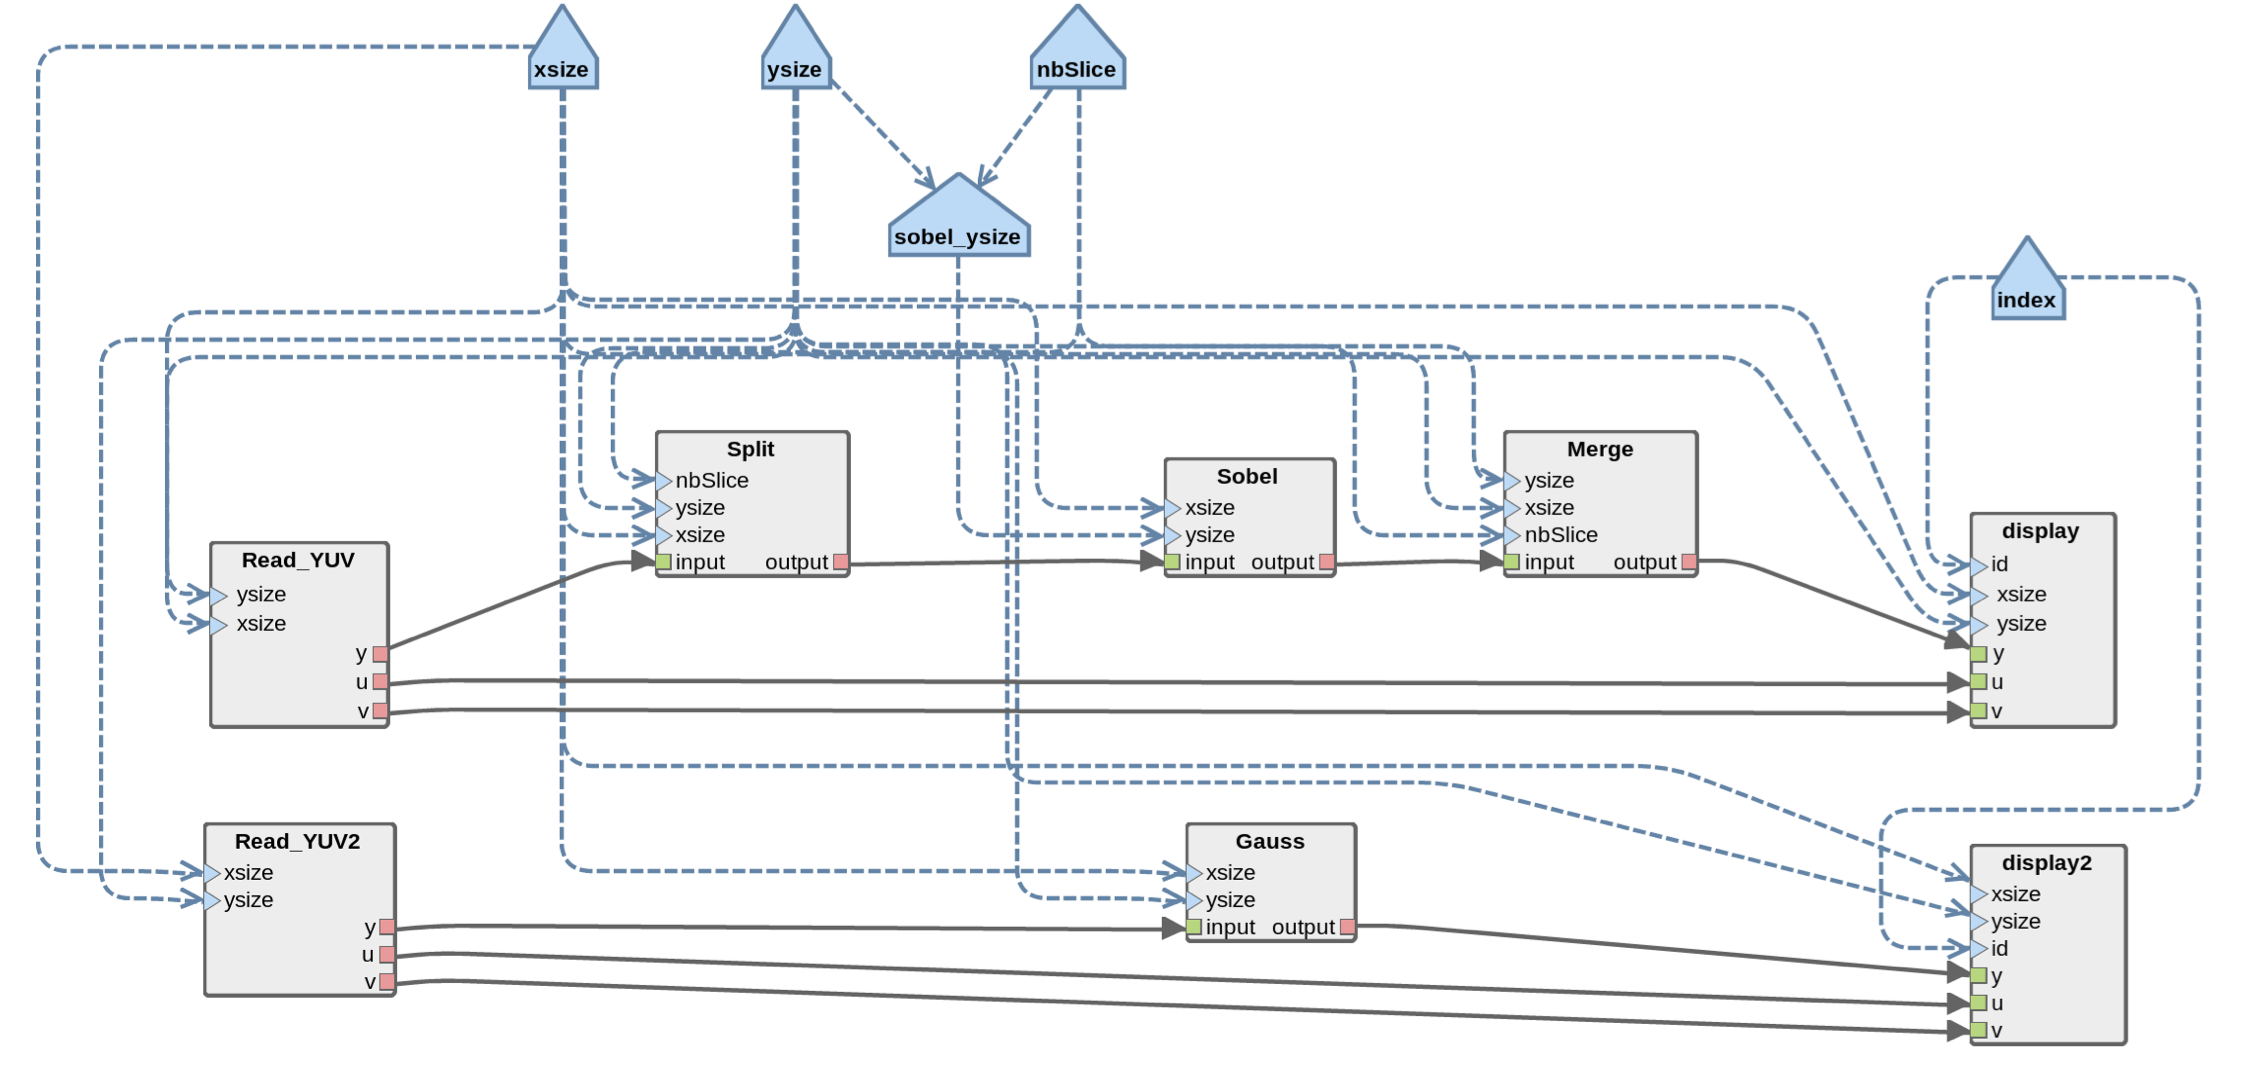
\includegraphics[width=1.3\textwidth,natwidth=2250,natheight=1090]{preesm_gauss.png}
\caption{A Sketch of The Video Filter Actor Network}\label{sketch}
\end{center}
\end{figure}
To keep the model simple and the program well analyzable all of the processing paths in the network are independent. The shared dependencies in the sketch (marked with dashed lines) are constants related to the video stream and will change in the actual application.

Each filter implemented will have its own independent processing path.

The first actors on each of the processing paths load the video frames form memory and pass them to splitting actors. The splitting actor splits the frames to suitable number of splices to enable processing of the same video stream on multiple cores. The filter actor follows the splitting actors. Partial frames filtered in the filter actor are merged in to whole frames in the merge actors. The last actors on each processing path are sink actors that collect data from the execution and frees resources.

The filter actors will be run on all cores according to manual selection before execution. The cores on which the other actors will run on are to be determined when more knowledge about the execution is available.

\subsection{Video Filter Application Using OpenEM}
The video filter application first constructed as a PREESM actor model, will be implemented using OpenEM. The actors in the actor model map to execution objects in a straightforward manner. An execution object is allocated for each actor in the actor model. The events passed between the actors encapsulate the data in the video streams.

In contrast to the PREESM application where the schedule has to be changed for each number of video streams, the OpenEM implementation will not be changed for the different workloads.

The specifics of setting up the execution objects, number of queues attached to them, the priority of the queues and other specifics depend heavily on the final workload application and thus are not further explained here. The details are also subject to change based on the initial measurements to make the workload better reflect a realistic application.
\subsection{Workload}
The workload application needs to be kept simpel to keep it analyzable. Complex parts of real applications unrelated to the parallel execution such as I/O are omitted from the workload implementation. Without I/O available the video streams need to be preloaded to the memory. CCS provides tools for preloading.

The purpose of the experiment is to understand the OpenEM behavior under dynamic load. Organizing the workload so that the number of streams could actually be dynamically changed at runtime will not be necessary if the cost of switching between streams can be estimated. A number of static loads will be constructed and measured on both of the applications.